\documentclass[11pt]{article}
\usepackage{alltt}
\usepackage[fleqn]{amsmath}
\usepackage{floatflt}
\usepackage{graphicx}
\usepackage{longtable}
\usepackage{srcltx}
\usepackage[strings]{underscore}

\textwidth 6.5in
\oddsidemargin -0.25in
%\evensidemargin -0.5in
\topmargin -0.5in
\textheight 9in

\newcommand{\docname}{\bf wvs-048r11}
\newcommand{\docdate}{9 June 2020}

\ifx\pdfoutput\undefined
  \pdfoutput=0
  \usepackage[hypertex,plainpages,hyperindex=true]{hyperref}
  \hypersetup{%
    hypertexnames=false%
  }
  % Specify the driver for the color package
  \ExecuteOptions{dvips}
  %\ExecuteOptions{xdvi}
\else
  \ifnum\pdfoutput>0
    \usepackage[pdftex,plainpages,hyperindex=true,pdfpagelabels]{hyperref}
    \hypersetup{%
      hypertexnames=false,%
      colorlinks=true,%
      linktocpage=true,%
    }
    % Specify the driver for the color package
    \ExecuteOptions{pdftex}
  \else
    \usepackage[hypertex,plainpages,hyperindex=true]{hyperref}
    \hypersetup{%
      hypertexnames=false%
    }
    % Specify the driver for the color package
    \ExecuteOptions{dvips}
    %\ExecuteOptions{xdvi}
  \fi
\fi

\hyperbaseurl{}
\newcommand\hr[1]{\href{#1.dvi}{dvi}, \href{#1.pdf}{pdf}}
\newcommand\h[1]{#1 (\hr{#1})}

\begin{document}

%\tracingcommands=1
\newlength{\hW} % heading box width
\newlength{\pW} % page number field width
\settowidth{\hW}{\docname}
\settowidth{\pW}{Page \pageref{lastpage}\ of \pageref{lastpage}}
\ifdim \pW > \hW \setlength{\hW}{\pW} \fi
\makeatletter
\def\@biblabel#1{#1.}
\newcommand{\ps@twolines}{%
  \renewcommand{\@oddhead}{%
    \docdate\hfill\parbox[t]{\hW}{{\hfill\docname}\newline
                          Page \thepage\ of \pageref{lastpage}}}%
\renewcommand{\@evenhead}{}%
\renewcommand{\@oddfoot}{}%
\renewcommand{\@evenfoot}{}%
}%
\makeatother
\pagestyle{twolines}

\vspace{-10pt}
\begin{tabbing}
\phantom{References: }\= \\
To: \>Bill\\
Subject: \>Different solution for $\phi$--$H$ calculation in {\tt metrics\_m}\\
From: \>Van Snyder\\
\end{tabbing}

\parindent 0pt \parskip 10pt
\vspace{-20pt}

\newcommand\Req{R^\oplus_{\text{eq}}}
\newcommand\Reqs{{\Req}_s}

\begin{floatingfigure}{3.65in}
{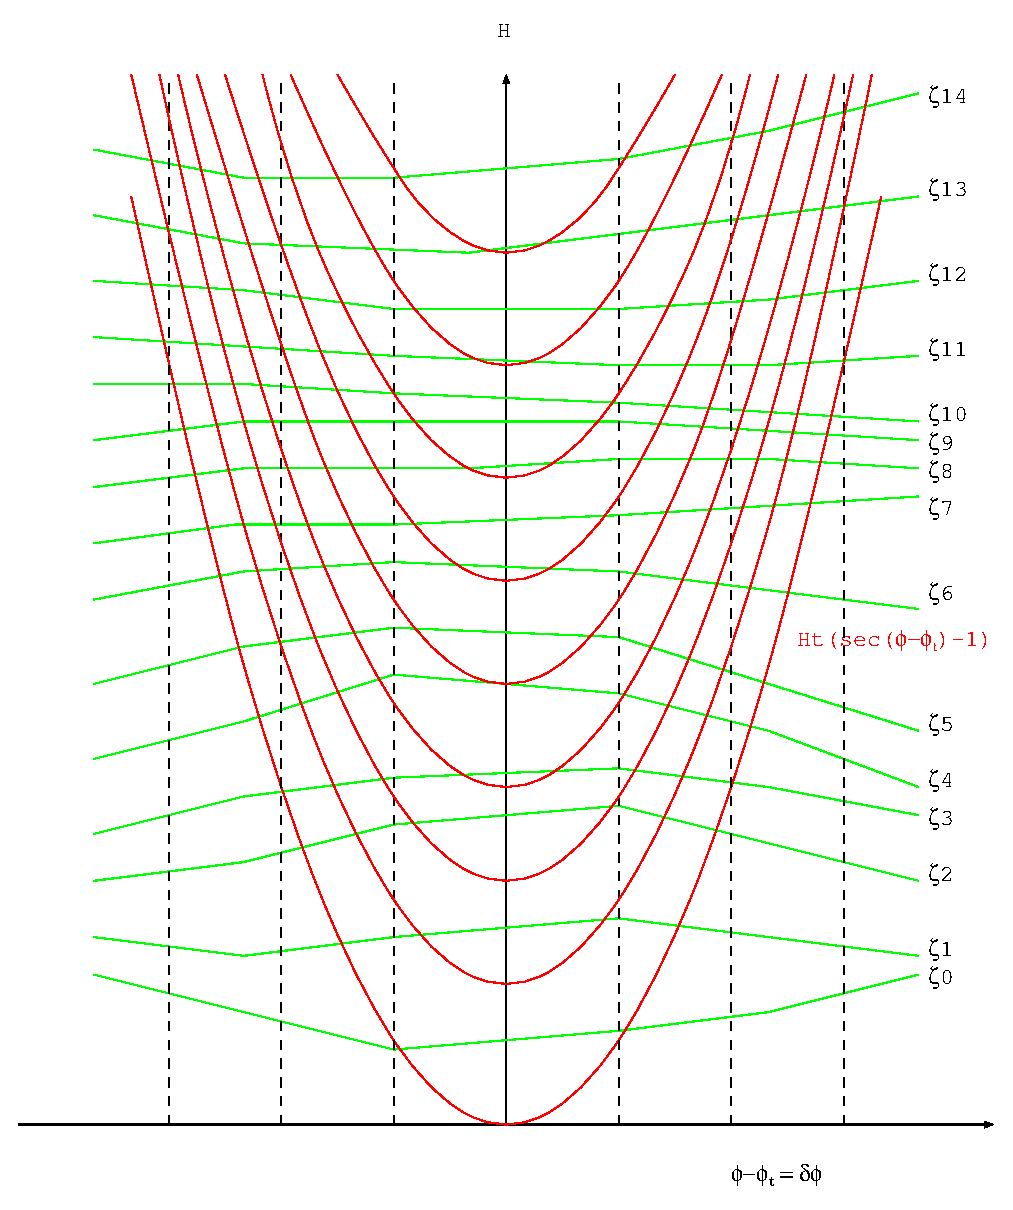
\includegraphics[width=3.5in,height=4.5in,clip]{./wvs-048-grid2}}
\end{floatingfigure}

We want to solve for $\phi$ and $H$ at the intersections of the line of
sight with constant-$\zeta$ surfaces.

Normally one thinks of the line of sight as a straight line, and
constant-$\zeta$ surfaces as approximate circles roughly concentric with
the earth.

This diagram shows the line of sight intersecting the constant-$\zeta$
surfaces in cartesian $\phi$--$H$ co\"{o}rdinates instead of polar 
$\phi$--$\zeta$ co\"{o}rdinates.  The heights on con\-stant-$\zeta$
surfaces are the green lines (straight lines because we use linear
interpolation in $\phi$, instead of approximate circles), the lines of
sight are the red lines (secant curves instead of straight lines), and the
temperature $\phi$ basis $\phi_1 \dots \phi_n$ is the vertical black
lines.  The quantity $H-\Req$, where $\Req$ is the equivalent circular
earth radius, is given at specified values of $\phi$ and $\zeta$, i.e., at
the intersections of the green and black lines, by the array {\tt
H\_ref}.  The tangent angle $\phi_t$, the tangent height $H_t$, $\Req$,
$\zeta_1\dots\zeta_m$, and $\phi_1 \dots \phi_n$ are given.

Denote {\tt H\_ref} by $H_{ij}$.  Each row of {\tt H\_ref} gives the
endpoints of piecewise-linear heights on a con\-stant-$\zeta$ surface. 
Writing the intersection of that line with the line of sight expressed as
a function of $\phi$, \emph{viz.}\ $H = H_t \sec \phi$, interpolating $H$
linearly in $\phi$ between $H_{ij}$ and $H_{i,j+1}$, using $H_\text{tan} =
H_t - \Req$, and subtracting $H_t$ from both sides to cancel $\Req$ on the
left side, we need to solve

\begin{equation}\begin{split}\label{one}
H_{ij} + \Req + (H_{i,j+1}-H_{ij})
                  \frac{\phi-\phi_j}
                       {\phi_{j+1}-\phi_j} -
                  ( H_\text{tan} + \Req ) \,&= \\
H_{ij} + (H_{i,j+1}-H_{ij})
                  \frac{\phi-\phi_j}
                       {\phi_{j+1}-\phi_j} -
                  H_\text{tan} \,&= \\
H_{ij} + (H_{i,j+1}-H_{ij})
                  \frac{(\phi-\phi_t)-(\phi_j-\phi_t)}
                       {\phi_{j+1}-\phi_j} -
                  H_\text{tan} \,&=
H_t(\sec ( \phi - \phi_t ) - 1) \\
\end{split}\end{equation}

for $\phi$ when $\phi_1 \leq \phi \leq \phi_n$, where $n$ is the number
of columns in {\tt H\_ref}, for all $i$ and $j$.  For $\phi < \phi_1$ or
$\phi > \phi_n$ assume constant-$\zeta$ surfaces are also constant-$H$
surfaces, i.e., $H_{i0} = H_{i1}$ and $H_{in} = H_{i,n+1}$, which reduces
the above to $H_{i0} = H_t \sec(\phi-\phi_t)$ or $H_{in} = H_t
\sec(\phi-\phi_t)$.

An added complication is that we refer all measurements to the one bar
pressure surface $H_s$, which is gotten by interpolating $H_{1,1\dots n}$
or a given array of surface heights to $\phi_t$.  Using $H_{ts} =
H_\text{tan} - H_s$, $\Reqs = \Req + H_s$, $H_t = H_{ts} + \Reqs$, adding
and subtracting $H_s$ from its left side, and using $H^-_{ij} =
H_{ij}-H_s$ etc., Equation (\ref{one}) becomes

\begin{equation}\label{two}
H^-_{ij} + (H^-_{i,j+1}-H^-_{ij})
                  \frac{(\phi-\phi_t)-(\phi_j-\phi_t)}
                       {\phi_{j+1}-\phi_j} -
                  H_{ts} =
H_t(\sec ( \phi - \phi_t ) - 1)\,.
\end{equation}

The angle $\phi_t$ is the one for the ray segment being calculated.  For
Earth-reflecting rays, the tangent points on the incident and reflected
segments are different by $2 \cos^{-1} \frac{H_t}\Reqs$.

We write Equation (\ref{two}) as a zero-finding problem

\begin{equation}\label{three}
d(\delta\phi) = a\, (\sec\delta\phi-1) + b\, \delta\phi + c = 0
\end{equation}

where

\begin{equation}\begin{split}
\delta\phi =\,& \phi - \phi_t\,, \,\, \Delta\phi = \phi_{j+1}-\phi_j\\
a =\,& H_t \Delta\phi\,, \\
b =\,& -(H^-_{i,j+1}-H^-_{ij}) = -(H_{i,j+1}-H_{ij})
   \text{ (}H_s\text{ cancels here), and} \\
c =\,& \phi_j (H^-_{i,j+1}-H_{ts}) -\phi_{j+1} (H^-_{ij}-H_{ts})
   + b\,\phi_t \\
  =\,& H^-_{i,j+1} ( \phi_j - \phi_t ) - H^-_{ij} ( \phi_{j+1}-\phi_t )
   + H_{ts} \Delta\phi\,. \\
\end{split}\end{equation}

To start a Newton iteration to solve Equation(\ref{three}), use
$\sec\delta\phi \approx 1 + \frac12 \delta\phi^2$, and solve for
$\delta\phi$ in

\begin{equation}
 \frac12 a\, \delta\phi^2 + b \, \delta\phi + c = 0\,.
\end{equation}

To the left of the tangent point, choose the minimum of the two
solutions; otherwise, choose the maximum.  This potentially has two
solutions at the tangent point unless the tangent point is at one of the
reference $\zeta$ values.  The existing code forces $\delta\phi$ to be
zero at the tangent.  If this has complex roots, or $\delta\phi < \phi_j$
or $\delta\phi > \phi_{j+1}$, assume $b=0$ and use $\delta\phi = \cos^{-1}
\frac{2 H_t}{H_{ij}+H_{i,j+1}}$.

When $|\delta\phi| < 0.2$ radians use an $8^\text{th}$-order polynomial

\begin{equation}
\sec\delta\phi - 1 \approx P_8(\delta\phi) =
 \frac12 \delta\phi^2 + \frac5{24} \delta\phi^4
 + \frac{61}{720} \delta\phi^6 + \frac{277}{8064} \delta\phi^8
\end{equation}

to approximate $\sec \delta \phi -1$ because the latter suffers
cancellation when $\delta\phi \approx 0$, giving

\begin{equation}
a\, P_8(\delta\phi) + b\, \delta\phi + c \approx 0\,.
\end{equation}

Using 16-digit arithmetic, $-1.5 \times 10^{-9} < P_8(\delta\phi) -
\sec(\delta\phi) + 1 \leq 0$ for $|\delta\phi| \leq 0.2$.

For the Newton iteration $\delta\phi_{n+1} = \delta\phi_n - d(\delta\phi_n) /
d^\prime(\delta\phi_n)$, the derivatives

\begin{equation}
d^\prime(\delta\phi) = a\, \sec \delta\phi \tan \delta\phi + b \approx
 P_8^\prime(\delta\phi) + b
\end{equation}

are necessary.  Remember, $\tan\delta\phi = \text{signum}(\delta\phi)
\sqrt{\sec^2 \delta\phi - 1}$, not simply $\left|\sqrt{\sec^2 \delta\phi -
1}\right|$.

\label{lastpage}
\end{document}
% $Id$

% $Log$
% Revision 1.11  2020/04/14 22:45:41  vsnyder
% Remove .eps from graphic filename because pdflatex wants to convert it itself
%
% Revision 1.10  2012/03/30 20:41:42  vsnyder
% Repair graphics stuff
%
% Revision 1.9  2009/05/12 23:41:09  vsnyder
% Remark about different tangent angles for incident and reflected rays, more cleanup
%
% Revision 1.8  2009/04/30 23:34:53  vsnyder
% Need abs around 'delta phi'
%
% Revision 1.7  2009/04/30 02:45:11  vsnyder
% Write Newton iteration correctly
%
% Revision 1.6  2009/04/30 02:40:29  vsnyder
% Correct a sign error, derivatives
%
% Revision 1.5  2009/04/29 22:35:08  vsnyder
% Clarify and simplify
%
% Revision 1.4  2009/04/28 02:55:18  vsnyder
% Make notation more consistent
%
% Revision 1.3  2009/04/28 00:41:58  vsnyder
% Undo erroneous sign change - wvs-048r2 is correct
%
